% --------------------------------------------------------------
% This is all preamble stuff that you don't have to worry about.
% Head down to where it says "Start here"
% --------------------------------------------------------------
 
\documentclass[12pt]{article}
 
\usepackage[margin=1in]{geometry} 
\usepackage{amsmath,amsthm,amssymb}
\usepackage{listings}
\usepackage{enumitem}   
\usepackage{graphicx}
\graphicspath{ {./images/} }

\lstset{
   basicstyle=\fontsize{8}{9}\selectfont\ttfamily
}
 
\newcommand{\N}{\mathbb{N}}
\newcommand{\Z}{\mathbb{Z}}
 
\newenvironment{theorem}[2][Theorem]{\begin{trivlist}
\item[\hskip \labelsep {\bfseries #1}\hskip \labelsep {\bfseries #2.}]}{\end{trivlist}}
\newenvironment{lemma}[2][Lemma]{\begin{trivlist}
\item[\hskip \labelsep {\bfseries #1}\hskip \labelsep {\bfseries #2.}]}{\end{trivlist}}
\newenvironment{exercise}[2][Exercise]{\begin{trivlist}
\item[\hskip \labelsep {\bfseries #1}\hskip \labelsep {\bfseries #2.}]}{\end{trivlist}}
\newenvironment{reflection}[2][Reflection]{\begin{trivlist}
\item[\hskip \labelsep {\bfseries #1}\hskip \labelsep {\bfseries #2.}]}{\end{trivlist}}
\newenvironment{proposition}[2][Proposition]{\begin{trivlist}
\item[\hskip \labelsep {\bfseries #1}\hskip \labelsep {\bfseries #2.}]}{\end{trivlist}}
\newenvironment{corollary}[2][Corollary]{\begin{trivlist}
\item[\hskip \labelsep {\bfseries #1}\hskip \labelsep {\bfseries #2.}]}{\end{trivlist}}
 
\begin{document}
 
% --------------------------------------------------------------
%                         Start here
% --------------------------------------------------------------
 
%\renewcommand{\qedsymbol}{\filledbox}
 
\title{Homework 4}%replace X with the appropriate number
\author{Hai Nguyen \& Huan Nguyen\\ %replace with your name
STAT760 - Statistical Learning} %if necessary, replace with your course title
\maketitle
\textbf{Problem 1}
\\Divide the data into a train a and a test set. Train a logistic regression predictor for chd using from one to eight predictors (write your own linear regression function). Graph the test error for the eight possible regressions.\\
\textit{Matlab code:}
\begin{lstlisting}
clc
close all
A = load('data_processed.txt');
n = length(A);
test_idx = round(0.7 * n);
Y_train = A(1:test_idx-1,11);
Y_test = A(test_idx:end,11);
alpha = 0.00001;
epsilon = 0.00001;
train_likelihood = [];
test_likelihood = [];
for i=1:8
    X_train = A(1:test_idx-1,2:i+1);
    m_train = mean(X_train);
    s_train = std(X_train);
    X_train = (X_train - m_train)./s_train;
    X_train = [ones(test_idx-1,1) X_train];
    X_train_scale = X_train;
    beta = rand(i+1,1);
    pre_cost = 0;
    cost = 100;
    itr = 1;
    while(abs(cost - pre_cost) > epsilon)
        pre_cost = cost;
        prop = exp(X_train*beta)./(1+exp(X_train*beta));
        for j=1:test_idx-1
            X_train_scale(j,:) = X_train(j,:)*(Y_train(j)-prop(j));
        end
        beta = beta + alpha*sum(X_train_scale,1)';
        cost = Y_train'*X_train*beta - sum(log(1+exp(X_train*beta)));
        %fprintf('Iter:%d, cost:%d\n',itr,cost);
        itr = itr + 1;
    end
    fprintf('Number of predictor:%d, iter:%d, training likelihood:%d\n',i,itr,exp(cost));
    train_likelihood = [train_likelihood exp(cost)];
    %Test error
    X_test = A(test_idx:end,2:i+1);
    X_test = (X_test - m_train)./s_train;
    X_test = [ones(n-test_idx+1,1) X_test];    
    test_cost = Y_test'*X_test*beta - sum(log(1+exp(X_test*beta)));
    test_likelihood = [test_likelihood exp(test_cost)];
    fprintf('Test likelihood:%d\n',exp(test_cost));
end
figure
%plot(train_likelihood,'b');hold on
plot(test_likelihood,'r')
title('Test error')
grid on
%legend('train likelihood','test likelihood')
\end{lstlisting} 
\begin{figure}[h!]
\begin{center}
  \caption{Test likelihood with different number of predictors}
  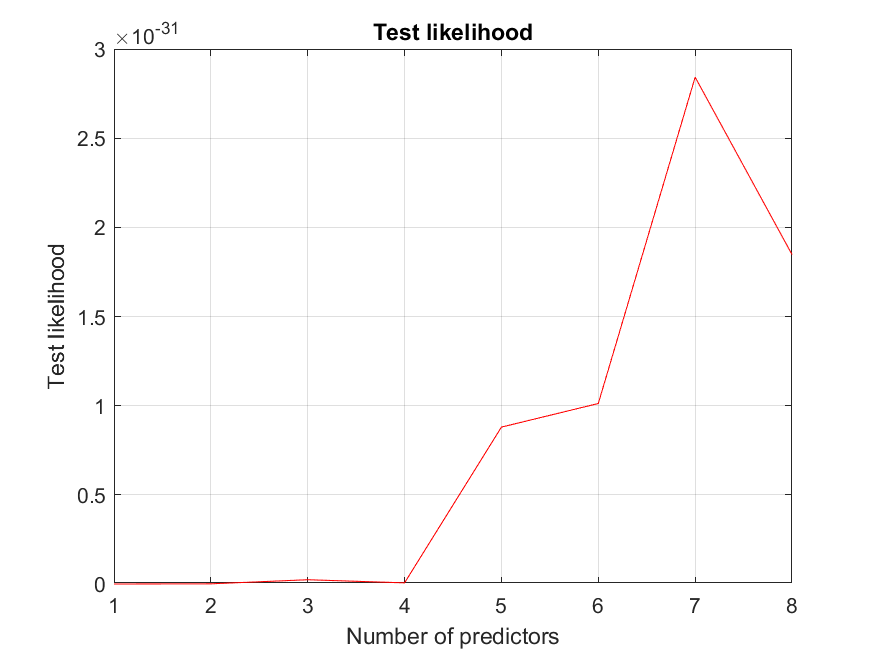
\includegraphics[width=1\textwidth]{images/HW4.png}
 \end{center}
\end{figure}
\textbf{Problem 2}
\begin{enumerate}
    \item Using a little bit of algebra, prove that (4.2) is equivalent to (4.3). In other words, the logistic function representation and logit representation for the logistic regression model are equivalent.
    \\ \textit{We have}
    \begin{align*}
        p(X) = \frac{e^{\beta_0 + \beta_1X}}{1 + e^{\beta_0 + \beta_1X}}
        \\\rightarrow e^{\beta_0 + \beta_1X}(1-p(X)) = p(X)
        \\\rightarrow \frac{p(X}{1-p(X)}=e^{\beta_0 + \beta_1X}
    \end{align*}
    \item It was stated in the text that classifying an observation to the class for which (4.12) is largest is equivalent to classifying an observation to the class for which (4.13) is largest. Prove that this is the case. In other words, under the assumption that the observations in the $k_{th}$ class are drawn from a N ($\mu_k$ , $\sigma^2$ ) distribution, the Bayes’ classifier assigns an observation to the class for which the discriminant function is maximized.
    \\\textit{To use the Bayes classifier, we have to find the class $k$ for which
    \begin{equation*}
        p_k(x) = \frac{\pi_k\frac{1}{\sqrt{2\pi}\sigma}e^{-\frac{1}{2\sigma^2}(x - \mu_k)^2}}{\sum_{l = 1}^K\pi_l\frac{1}{\sqrt{2\pi}\sigma}e^{-\frac{1}{2\sigma^2}(x - \mu_l)^2}} = \frac{\pi_ke^{-\frac{1}{2\sigma^2}(x - \mu_k)^2}}{\sum_{l = 1}^K\pi_le^{-\frac{1}{2\sigma^2}(x - \mu_l)^2}}
        \end{equation*}
    is largest, which is equivalent to find $k$ such that:
    \begin{equation*}
        \log p_k(x) = \log (\pi_k) -\frac{1}{2\sigma^2}(x - \mu_k)^2 - \log \sum_{l = 1}^K\pi_le^{-\frac{1}{2\sigma^2}(x - \mu_l)^2}
    \end{equation*}
    is largest. As the last term is independent of $k$, it is equivalent to find $k$ for which
    \begin{equation*}
        \log (\pi_k) -\frac{1}{2\sigma^2}(x - \mu_k)^2 = \log(\pi_k) - \frac{x^2}{2\sigma^2} + \frac{\mu_k}{\sigma^2}x - \frac{\mu_k^2}{2\sigma^2}
    \end{equation*}
    is largest. The term in $x^2$ is independent of $k$, so it remains to find $k$ for which:
    \begin{equation*}
        \delta_k(x) = \frac{\mu_k}{\sigma^2}x - \frac{\mu_k^2}{2\sigma^2} + \log(\pi_k)
    \end{equation*}
    is maximized (this is the discriminant function).}
\end{enumerate}

% --------------------------------------------------------------
%     You don't have to mess with anything below this line.
% --------------------------------------------------------------
 
\end{document}